\documentclass[dvipdfmx,uplatex]{jsarticle}
\usepackage{../macros}



\begin{document}
\subsection{Maxwell方程式}
\begin{law}
\begin{align}
\nabla \cdot \vec{E} &= \dfrac{\rho}{\varepsilon}\\
\nabla \cdot \vec{B} &= 0\\
\nabla \times \vec{E} &= -\dfrac{\partial \vec{B}}{\partial t}\\
\nabla \times \vec{B} &= \mu\varepsilon \dfrac{\partial \vec{E}}{\partial t} + \mu\vec{j}
\end{align}
\end{law}

\subsubsection{Gaussの法則}
\begin{law}
\[
\int_S \bm{E} \cdot \bm{n} ds = \frac{Q}{\varepsilon _0}
\]
\end{law}

\subsubsection{Amp\`{e}reの法則}
\begin{law}[アンペールの法則] \mbox{}\\
閉回路上の磁場の大きさの総和は閉回路を貫く総電流に等しい. \\
すなわち
\[
\oint_{\partial S} \bm{H} \cdot d \bm{l} = \int_S \bm{J} \cdot d \bm{S} = I \\
\]
ただし、\\
H	: 磁場の強さ,
J	: 電流密度,
I	: 積分領域 S を貫く総電流,
dl	: 線素ベクトル,
dS	: 面素ベクトル,
$\partial S$	: 面Sの境界 \\
\end{law}
またこれゆえに
\[
\mathrm{rot} \bm{H} = \nabla \times \bm{H} = \bm{J} \\
\]
\begin{theo}
無限に長い直線電流が距離$r$の位置に成す磁場の大きさ$H$は
\[
H = \frac{I}{2 \pi r}
\]
\end{theo}
\begin{proof}
\[
\oint_S  \bm{H} \cdot d \bm{l} = 2 \pi r = I
\]
\end{proof}

\subsubsection{Faradayの電磁誘導の法則}
\begin{law}
\[
V = -N \frac{\Delta \Phi}{\Delta t} \\
\]
(Nは巻き数)\\
さらに
\[
\oint_S \bm{E} \cdot d\bm{s} = - \frac{d \Phi _B}{dt}\\
\]
\[
\nabla \times \bm{E} = - \frac{\partial \bm{B}}{\partial t}
\]
\end{law}

\subsection{静電磁場}

\subsubsection{静電ポテンシャル}

\subsubsection{ポアソン方程式}

\subsubsection{定常電流}

\subsubsection{ビオ・サバールの法則}
\begin{law}[ビオ・サバールの法則] \mbox{} \\
微小な長さの電流要素$I d\bm{l} $から$ \bm{r} $離れた位置に作られる微小な磁場$ d\bm{H} $は
\[
d\bm{H} = \frac{Id\bm{l} \times \bm{r}}{4 \pi r^3} = \frac{Id\bm{l}}{4 \pi r^2} \times \frac{\bm{r}}{r} \\
\]
\end{law}
\begin{theo}
半径$r$の円電流の中心に生じる磁場の大きさ$H$は
\[
H = \frac{I}{2r}
\]
\end{theo}
\begin{proof}
\begin{align*}
H &= \left| \oint_I \frac{Id\bm{l} \times \bm{r}}{4 \pi r^3} \right| \\
&= \frac{I \times 2 \pi r^2}{4 \pi r^3} \\
&= \frac{I}{2r}
\end{align*}
\end{proof}

\newpage

\begin{theo}
$I \si{\ampere}$の電流が流れる,単位巻き数$n$ソレノイドコイル中心軸上の点における磁場の大きさ$H'$は \\
左右にコイルが長く続くとき,
\[
H' = nI
\]
コイルの端のとき,
\[
H' = \frac{nI}{2}
\]
\end{theo}
\begin{proof} 

\begin{figure}[htbp]
\begin{center}
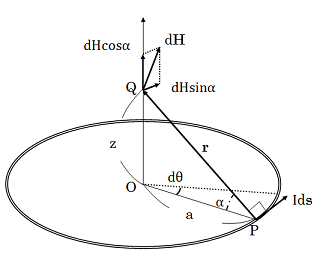
\includegraphics[width=100mm]{Biot-savart.png}
\end{center}
\end{figure}
上図で
\[
r = \sqrt{a^2 + z^2}, \cos \alpha = \frac{a}{r}
\]
である.\\
また
\[
\frac{\pi}{2} - \alpha = \beta
\]
とおく.(図の都合上このようにおいている) \\
$dH$の面に平行な成分$dH_{\parallel} = dH \sin \alpha$は等方性より周回積分すると$0$ に等しい.よって$dH_{\perp} = dH \cos \alpha$のみを考える.
\[
dH_{\perp} = \frac{1}{4 \pi} \frac{I \cos \alpha d\bm{l} \times \bm{r}}{r^3}
\]
ここで$dl = a d \theta$を用いて
\begin{align*}
H_{\perp} &= \int \frac{1}{4 \pi} \frac{I \cos \alpha a d\theta \times \bm{r}}{r^3} \\
(&= \oint_I dH_{\perp}\cos \alpha ) \\
&= \frac{I}{4 \pi r^2} 2 \pi a \cos \alpha \\
&= \frac{I \cos^3 \alpha}{2a} \\
&= \frac{I \sin^3 \beta}{2a}
\end{align*}
(これより$z=0$のとき$H=\frac{I}{2a}$を得る.) \\
このことよりソレノイドコイルのうち$ndz$個のコイルが仰角$\alpha$方向に成す微小磁場$dH'$は
\begin{align*}
dH' = \frac{I \sin^3 \beta}{2a} \times n dz
\end{align*}
また
\begin{align*}
dz &= -\frac{r}{\sin^2 \beta} d \beta \\
\therefore dH' &= -\frac{nI}{2}\sin \beta d \beta
\end{align*}
以上より左右にコイルが長く続く点の磁場は
\[
H' = \int^{\pi}_{\beta = 0} dH' = nI
\]
コイルの端の点の磁場は
\[
H' = \int^{\frac{\pi}{2}}_{\beta = 0} dH' = \frac{nI}{2}
\]

\end{proof}

\subsubsection{アンペール力,ローレンツ力}

\subsubsection{コンデンサー}

\subsection{動電磁場}

\subsection{回路}

\subsubsection{キルヒホッフの法則}

\end{document}
